\documentclass[11pt]{article}

% ---------------------------------------------------------------------------
% Points Left on the Table -- arXiv preprint (DRAFT)
% Build:  pdflatex main && bibtex main && pdflatex main && pdflatex main
% ---------------------------------------------------------------------------

\usepackage[margin=1in]{geometry}
\usepackage[utf8]{inputenc}
\usepackage{amsmath,amssymb}
\usepackage{booktabs}
\usepackage{graphicx}
\usepackage{xcolor}
\usepackage{microtype}
\usepackage[numbers,sort&compress]{natbib}
\usepackage[colorlinks=true,allcolors=blue!55!black]{hyperref}
\usepackage{caption}
\captionsetup{font=small}

\graphicspath{{figures/}}

% A loud marker for the one result we are deliberately deferring to the 208-game run.
\newcommand{\TODO}[1]{\textcolor{red}{\textbf{[TODO: #1]}}}
\newcommand{\plot}{\textsc{plot}}
\newcommand{\epv}{\textsc{epv}}
\newcommand{\xpts}{\textsc{xPoints}}

\title{\textbf{Points Left on the Table}\\[2pt]
\large An open expected-points value layer and an outcome-validated\\
decision-regret metric for NBA tracking data}

\author{Jake Parker\thanks{Independent researcher. Correspondence: \texttt{jakeparkeremail@gmail.com}.
Code and reproduction: \url{https://github.com/jparker2006/PLOT}.}}

\date{\today}

\begin{document}
\maketitle

\begin{abstract}
The box score records what a basketball player \emph{did}; it is structurally blind to the quality of
the \emph{decisions} that produced it. We build, on the only frozen public season of NBA optical
tracking (2015--16), an open per-action expected-points value layer (an \epv{} ``eval bar'') and use
it to define \plot{} (``Points Left On the Table''): a per-decision \emph{regret} --- the gap between
the expected points of the best genuinely-available option and the option the player chose, scored by
the model's expected value rather than the realized outcome, so it measures decision quality and not
luck. We validate the pipeline through a sequence of pre-registered gates: the value layer is
calibrated under leave-one-game-out cross-validation (log-loss $0.82$ vs.\ a $1.09$ constant baseline;
calibration-in-the-large $-0.011$; expected calibration error $0.063$ points); the one-step
counterfactual inputs are calibrated on held-out real continuations; and the resulting player metric
is split-half reliable (Spearman--Brown $0.68$), survives controls for shot location and finishing
skill, and is largely orthogonal to the box score (joint $R^2$ with true-shooting and usage $\approx0.07$).
The central question --- does ``points left'' predict anything \emph{real}, or only the model against
itself? --- is answered with two outcome-validity tests on 208 games. \emph{Declining your own open
look} costs real points: net of observables, team, and shot-clock pressure, passing up an open look
costs $\approx\!0.11$ points on an average look and $\approx\!0.19$ on a high-value one; declining a
\emph{bad} look is free; the cost grows monotonically with look value; and it survives removing
turnover exposure and action-layer mis-typing. The obvious selection objection cuts the wrong way:
decliners realize \emph{fewer} points than matched takers, not more, so on average the pass was not
concealing a better option the tracking missed. A second, counterintuitive finding comes from the
symmetric test --- \emph{shooting over a wide-open teammate} --- which does \emph{not} validate: the
teammate-kick counterfactual is flat in its modeled value and shooting over the open man realizes
\emph{more} points, not fewer. So \plot{} is outcome-valid precisely for the decision whose
counterfactual is directly observable (your own open shot), while the conventional ``pass to the open
man'' read is \emph{not} recoverable from public tracking --- whether because the open man is open
precisely \emph{because} he is not a threat, or because the teammate counterfactual is simply too crude
to score, the read is not one this data can credit. Both validations are at the \emph{decision} level; an out-of-sample cross-fit finds only \emph{weak, fragile}
support for clean attribution to individual \emph{players} (pooled within-role $r\!\approx\!0.11$,
heavily attenuated from an in-sample $0.33$, with one of two folds individually null), so we keep the
validated claim at the decision level and report player-level attribution as modest at best. A variance decomposition shows the between-player signal is majority within-role
decision quality ($52\%$) rather than role-of-touch ($29\%$), and the within-role component is itself
reliable and robust to the strength of the role control. We release the value layer, the metric, a
chess.com-style possession-review demo, and all gate code. We are explicit about scope: \plot{}
measures genuinely-left value \emph{conditional on observables}, not proven-causal ``decision IQ,'' and
the validated claim is narrow, modest in magnitude, and honest about selection on unobservables.
\end{abstract}

% ===========================================================================
\section{Introduction}
% ===========================================================================
A great pass that leads to a missed layup and a forced heave that happens to go in are recorded by the
box score in exactly the wrong order. Counting statistics --- and even the efficiency metrics built on
them --- evaluate \emph{outcomes}, which conflate decision quality with finishing skill and luck. Yet
coaches and analysts talk constantly about \emph{decisions}: the open shot a player passed up, the kick
to the corner he didn't make, the contested two he took over an open teammate. Player and ball tracking
make these decisions observable for the first time, but the dominant tracking-era value model ---
expected possession value (\epv{}) \citep{cervone2016multiresolution,cervone2014pointwise} --- stops
just short of scoring them. Cervone et al.\ introduced \epv{} and, alongside it, ``shot satisfaction''
(the value a shot adds relative to the possession's \epv{}): an essentially shot-centric, opposite-signed
cousin of regret. A possession-level \emph{regret} --- best genuinely-available option minus the chosen
one --- on \emph{public} data has remained a gap.

This paper closes part of that gap and is honest about the part it cannot. We make five contributions.

\begin{enumerate}
  \item \textbf{An open value layer.} A reproducible per-action expected-points model for NBA possessions
        --- a ``VAEP-for-basketball'' \citep{decroos2019actions} --- trained from public tracking, with a
        permutation-invariant set encoder over the ten players feeding a causal recurrent outcome head
        (\S\ref{sec:valuelayer}). It is calibrated on held-out games and its per-action $\Delta$\epv{}
        decomposition telescopes exactly to realized possession points.
  \item \textbf{The \plot{} regret metric.} A per-decision regret valued against the best
        genuinely-available alternative and scored by model expected value, aggregated to a per-player
        ``points left on the table'' (\S\ref{sec:plot}). We show it is a stable, distinct skill signal,
        not a relabeling of shot location, finishing, or the box score (\S\ref{sec:skill}).
  \item \textbf{Outcome validity at the decision level (the keystone).} Using realized possession
        outcomes as ground truth (\S\ref{sec:g6keystone}), declining your own open look costs real points
        in a dose-responsive way that survives every robustness cut we could devise. The natural
        selection objection cuts the \emph{wrong} way: decliners' realized outcomes are \emph{worse}, not
        better, than matched takers', so on average these passes were not justified by an unobserved
        superior option. These validations are at the decision level; an out-of-sample cross-fit gives
        only weak, fragile support for clean attribution to individual \emph{players} --- pooled
        within-role $r\!\approx\!0.11$, one of two folds null, heavily attenuated from an in-sample
        $0.33$ (\S\ref{sec:g6crossfit}).
  \item \textbf{The open-man myth (a finding in its own right).} The symmetric test ---
        \emph{shooting over a wide-open teammate} --- does \emph{not} validate: the teammate-kick
        counterfactual is flat in its modeled value, and shooting over the open man realizes \emph{more}
        points, not fewer (\S\ref{sec:g6asym}). Either an open man is often open precisely \emph{because}
        he is not a threat, or the teammate counterfactual is simply too crude to score from tracking
        (we cannot fully separate the two); either way the conventional ``pass to the open man'' read is
        not recoverable from public tracking. This is a result about the limits of what such tracking can
        credit, not merely a limit on \plot{}.
  \item \textbf{Artifacts.} The value layer, the metric, a chess.com-style possession-review web demo
        (\S\ref{sec:demo}), and the full gate-by-gate reproduction code are released openly.
\end{enumerate}

Throughout we treat the metric with deliberate skepticism. Every stage is a go/no-go gate, and the most
important gate (outcome validity) is the first one that is \emph{not} the model judged against itself.
We report a negative result (the teammate-kick test) as prominently as the positive one, because it is
what scopes the claim. And we are clear that the headline magnitude is modest --- declining a great open
look costs about a fifth of a point --- which is the honest size of a real, previously-unmeasured effect,
not a dramatic one.

% ===========================================================================
\section{Related work}
% ===========================================================================
\textbf{Expected possession value.} \epv{} \citep{cervone2016multiresolution} models a possession as a
multiresolution stochastic process and reads off the expected points conditional on the full
spatiotemporal state. It is the conceptual parent of our value layer. Our contributions relative to it
are (i) an open, lean reimplementation on public data, and (ii) building the possession-level regret
that \epv{} named but did not develop. \citet{sicilia2019deephoops} (DeepHoops) similarly evaluate
micro-actions with deep spatiotemporal features; we adopt that spirit with a smaller, calibration-first
model and an explicit decision metric on top.

\textbf{Action values in invasion sports.} VAEP \citep{decroos2019actions} values every soccer action as
the change in scoring/conceding probability it induces; our per-action $\Delta$\epv{} layer is the direct
basketball analog, with possession \epv{} playing the role of VAEP's state value.

\textbf{Shot quality and shooting strategy.} Shot-quality models such as qSQ/qSI
\citep{chang2014shotquality} estimate the value of a shot from its spatial context; we use a deliberately
lean ``\xpts{}'' shot model of the same family as the open-shot counterfactual. \citet{sandholtz2020markov,
sandholtz2020allocative} study shooting strategy and spatial allocative efficiency as decision problems;
our regret is a complementary, per-decision, outcome-validated quantity. Spatial-structure models of
offense and defense \citep{miller2014factorized,franks2015defense} inform our state features.

\textbf{Box-score baselines.} Efficiency and usage summaries \citep{kubatko2007starting} are the
incumbents we test \plot{} against for incremental information; the point of \plot{} is precisely to
measure something they cannot.

\textbf{Architecture.} The value layer uses a Deep Sets \citep{zaheer2017deepsets} encoder for
permutation invariance over players and a GRU \citep{cho2014gru} for the causal temporal head.

% ===========================================================================
\section{Data and possession pipeline}\label{sec:data}
% ===========================================================================
We use public 2015--16 NBA SportVU optical tracking: 25\,fps $(x,y)$ for ten players plus the 3D
ball, distributed through community archives \citep{linou2016movements} after the league's movement
endpoint was closed, merged with play-by-play (PBP) on \texttt{eventId == EVENTNUM} ($\approx\!98.5\%$
match). 2015--16 is the last season with publicly available league tracking; coverage runs
2015-10-27 through 2016-01-23 ($\approx$ half a season, $\approx\!636$ games). \textbf{We do not
re-host the raw data}: the repository ships a download script, derived features, and model outputs only,
with every transformation documented.

\textbf{Pipeline.} Each game is parsed to an internal schema and downsampled to 10\,fps parquet
(the model resolution; 25\,fps is retained only for demo clips). Possessions are segmented from PBP
event types plus the controlling team, terminating on a made field goal (with any and-one free throws),
defensive rebound, turnover, or period end; offensive rebounds \emph{continue} the possession. Realized
possession points are computed \emph{description-based} from the authoritative scorer team id, never from
the orientation-inconsistent and occasionally non-monotonic PBP \texttt{SCORE} column. Segmentation was
validated by exact points reconciliation on every local tracking game and on a 205-game PBP-only sweep
(a single residual traced to a known SCORE-column glitch).

\textbf{Orientation and quarantine.} Coordinates are canonicalized so offense always attacks the same
basket. Because the raw feed carries no possession orientation, we infer it from spatial evidence and
\emph{quarantine} games where the inference is not corroborated (single-confident-cell, conflicting, or
high-backcourt-fraction games), trading coverage for correctness. The headline corpus is the
\textbf{208 clean games} that pass all quality control; the value layer's calibration gate (G1) is
reported on a 10-game development subset for which both the baseline and sequence models were trained
under identical leave-one-game-out (LOGO) folds. We note one caveat the trade-off carries: the retained
games are not guaranteed missing-at-random --- if particular arenas or camera installations produced
systematically noisier tracking and were dropped, the clean corpus may be mildly non-representative of
the league (\S\ref{sec:limits}).

\textbf{Nested corpora.} The analysis uses several samples; Table~\ref{tab:corpora} names them and the
gate each serves, so the reader need not reverse-engineer which $N$ applies where. Development subsets
validate the machinery; the 208-game clean corpus carries the headline results.

\begin{table}[h]
\centering
\caption{\textbf{Nested corpora} and the gate each serves.}
\label{tab:corpora}
\small
\begin{tabular}{@{}lll@{}}
\toprule
Sample & Size & Used for \\
\midrule
Available half-season & $\approx\!636$ games & full public 2015--16 coverage (Oct 27 -- Jan 23) \\
Development subset     & 10 games (LOGO)      & value-layer + counterfactual calibration (G1, G2) \\
Development corpus     & 42 games             & validity method checks (G5) \\
\textbf{Headline corpus} & \textbf{208 clean games} & stability, distinctness, decomposition, validity (G3--G6) \\
Player panel           & 374--387 players     & $\ge\!30$ decisions; 374 matched to season box stats (G4) \\
\bottomrule
\end{tabular}
\end{table}

% ===========================================================================
\section{The value layer: an open expected-points model}\label{sec:valuelayer}
% ===========================================================================
The value layer predicts, at every frame of a possession, the distribution over the points the
possession will ultimately yield, $P(\text{points}=k)$ for $k\in\{0,1,2,3\}$, and reads off the
\textbf{eval bar}
\begin{equation}
  \epv{}_t \;=\; \sum_{k\in\{0,1,2,3\}} k \cdot P(\text{points}=k \mid \text{state}_t).
\end{equation}
We build two models with the \emph{identical} target, weighting, calibration code, and quarantine, so the
upgrade is an apples-to-apples comparison.

\textbf{Baseline (LightGBM).} A gradient-boosted multiclass head over coarse per-frame features
(canonical ball geometry, court region, game/shot clock, score margin, period, paint counts,
ball-handler-to-nearest-defender pressure). It is deliberately decision-insensitive --- a location/context
prior --- and exists to validate the calibration plumbing.

\textbf{Sequence model.} A permutation-invariant \textbf{Deep Sets} \citep{zaheer2017deepsets} encoder over
the ten players (offense/defense-masked mean+max pooling; per-player features are canonical position,
team and ball-handler flags, and distance to the ball), concatenated with a ball token and context vector,
fed to a \textbf{causal (unidirectional) GRU} \citep{cho2014gru} (hidden size 128, one layer) and a
per-frame multiclass head. Causality is a tested invariant: editing frame $t$ leaves all earlier frames'
predictions bit-identical, so the eval bar at time $t$ never peeks ahead. Training is on Apple MPS in
minutes per fold.

\textbf{Calibration (Gate G1).} Both models are evaluated out-of-fold on held-out \emph{games}
(Table~\ref{tab:g1}). The sequence model is well calibrated (calibration-in-the-large $-0.011$, moment
slope $0.955$ with $95\%$ CI $[0.92,0.99]$, expected calibration error $0.063$ points) and improves
log-loss, Brier, and the ordinal ranked probability score by $\approx\!17$--$21\%$ over the baseline, and
far over a constant-rate prior. We report the calibration slope as a diagnostic, not a gate; the gate is
(beats-constant-baseline) $\wedge$ (calibration-in-the-large) $\wedge$ (ECE). \textbf{G1 passes.}

\begin{table}[t]
\centering
\caption{\textbf{Gate G1 --- value-layer calibration}, leave-one-game-out on 10 development games
($\approx$\,$3.1$--$3.2\times10^5$ held-out frames). Lower is better for log-loss/Brier/RPS;
calibration-in-the-large (CITL) and ECE near $0$; slope near $1$. The sequence model is the eval bar used
downstream.}
\label{tab:g1}
\small
\begin{tabular}{lcccccc}
\toprule
Model & log-loss & Brier & RPS & CITL & ECE (pts) & slope \\
\midrule
Constant-rate prior      & 1.086 & 0.615 & 0.597 & ---     & ---   & ---   \\
Baseline (LightGBM)      & 1.014 & 0.569 & 0.545 & $+0.006$ & 0.054 & 1.15  \\
\textbf{Sequence (Deep Sets + GRU)} & \textbf{0.819} & \textbf{0.461} & \textbf{0.428} & $-0.011$ & 0.063 & 0.955 \\
\bottomrule
\end{tabular}
\end{table}

\textbf{Per-action decomposition.} Following VAEP \citep{decroos2019actions}, each on-ball action is
valued as $\text{value}(a) = \epv{}(\text{end}) - \epv{}(\text{start})$, grounded in the ball-handler
trace, with the terminal action pinned to realized points. By construction the action values telescope to
(realized points $-$ initial \epv{}) over a possession: across 1{,}774 possessions and 9{,}850 actions the
maximum absolute telescoping residual is exactly $0.0$. The action-type means are sensible
(Figure~\ref{fig:actionvalues}): made shot $+0.84$, foul drawn $+0.15$, pass $-0.05$ (mean $\approx 0$,
as a pass should be on average), missed shot $-0.47$, turnover $-0.54$.

\begin{figure}[t]
\centering
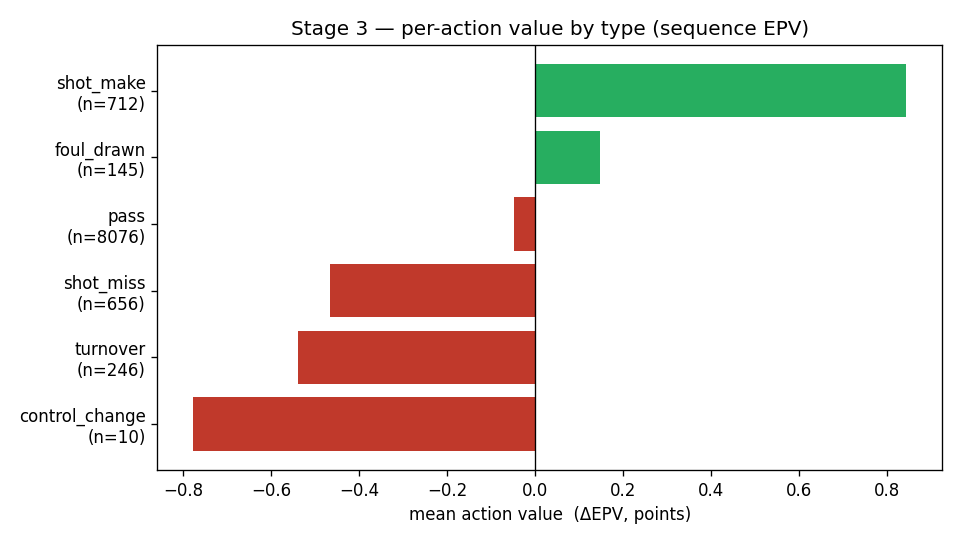
\includegraphics[width=0.62\linewidth]{action-value-by-type.png}
\caption{Per-action $\Delta$\epv{} by action type. The decomposition telescopes exactly to realized
possession points; signs and magnitudes are face-valid.}
\label{fig:actionvalues}
\end{figure}

% ===========================================================================
\section{The PLOT regret metric}\label{sec:plot}
% ===========================================================================
\textbf{Decision points and the available set.} We score decisions at action boundaries. The narrowest,
best-identified decision --- and the v1 metric --- is the \emph{open pass-up}: a ball-handler with no
defender within 4\,ft who passes rather than shoots. The \emph{best available} option is that open
shot, valued by an \xpts{} model; the \emph{chosen} value is the post-pass \epv{} read from the value
layer. Regret is
\begin{equation}
  \text{regret} \;=\; \underbrace{\xpts{}(\text{open shot here})}_{\text{best available}} \;-\;
  \underbrace{\text{\epv{}}(\text{chosen action})}_{\text{chosen, by model EV}},
\end{equation}
reported both clipped, $\max(0,\cdot)$ (``points left''), and signed (a diagnostic). Crucially the chosen
action is scored by its \emph{model expected value}, not its realized outcome: \plot{} measures the
decision, not whether it happened to work.

\textbf{The \xpts{} counterfactual model.} $\xpts{} = P(\text{make}\mid \text{distance, openness, shot
type})\times\text{points}$ is a regularized logistic model fit on observed shots --- well-identified
because it is trained on real shots from similar states. It uses a population make model with \emph{no}
shooter identity, so regret cannot smuggle in finishing skill (verified in \S\ref{sec:skill}).

\textbf{Gate G2 (one-step counterfactual calibration).} Regret is only meaningful if its two inputs are
calibrated on held-out \emph{real continuations}. They are (Table~\ref{tab:g2}): when the open shot
\emph{was} taken, \xpts{} matches realized points (calibration-in-the-large $+0.002$, ECE $0.077$, and it
beats a make-rate baseline on log-loss); when a pass \emph{was} made, post-pass \epv{} matches realized
outcomes (calibration-in-the-large $-0.014$, slope $0.915$, ECE $0.066$). \textbf{G2 passes}; regret is
not a calibration artifact.

\begin{table}[t]
\centering
\caption{\textbf{Gate G2 --- counterfactual inputs}, calibrated against held-out realized outcomes.}
\label{tab:g2}
\small
\begin{tabular}{lccccc}
\toprule
Input & $n$ & CITL & ECE (pts) & slope & beats baseline \\
\midrule
\xpts{} (open shot, when taken) & 1{,}233 & $+0.002$ & 0.077 & 0.842 & yes (log-loss $0.668{<}0.689$) \\
post-pass \epv{} (when passed)  & 8{,}076 & $-0.014$ & 0.066 & 0.915 & --- \\
\bottomrule
\end{tabular}
\end{table}

We later (\S\ref{sec:g6}) broaden the scored set to a \emph{credible set} that adds shot-selection
decisions (shooting over a wide-open, reachable, completion-discounted teammate), and analyze both the
metric's composition and its outcome validity on that set.

% ===========================================================================
\section{Is it a skill? Stability, distinctness, validity}\label{sec:skill}
% ===========================================================================
\textbf{Gate G3 (stable and not finishing).} On 208 games (124{,}953 open pass-up decisions, 380 players
with $\ge 30$), \plot{} is split-half reliable: splitting the season's games odd/even and correlating
per-player means gives Pearson $0.51$ ($p\!\approx\!0$), Spearman--Brown full-data reliability $0.68$
(Figure~\ref{fig:g3}). A nested OLS shows player identity explains regret \emph{beyond} shot location
($F(380,124568)=4.96$, $p\!\approx\!0$), and per-player regret is uncorrelated-to-mildly-negative with
finishing skill (Pearson $-0.17$), so it is not a relabeled finishing metric. \textbf{G3 passes.}

\textbf{Gate G4 (incremental over the box score).} On 374 players matched to season box statistics,
\plot{} is essentially unrelated to true-shooting ($r=+0.09$, n.s.) and only weakly related to usage
($-0.24$), points per game ($-0.21$), and field-goal attempts ($-0.24$). A joint regression on
true-shooting and usage explains just $R^2=0.075$ of \plot{} variance --- $>\!90\%$ is \emph{not} in the
box score (Figure~\ref{fig:g4}). \textbf{G4 passes} (incremental $\wedge$ reliable).

\begin{figure}[t]
\centering
\begin{minipage}{0.48\linewidth}\centering
  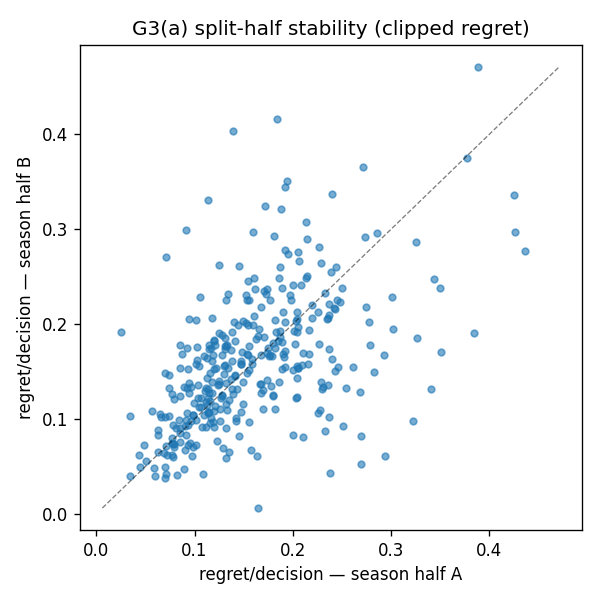
\includegraphics[width=\linewidth]{g3-split-half-scatter.png}
  \caption{G3: split-half reliability of per-player \plot{} across odd/even game halves.}
  \label{fig:g3}
\end{minipage}\hfill
\begin{minipage}{0.48\linewidth}\centering
  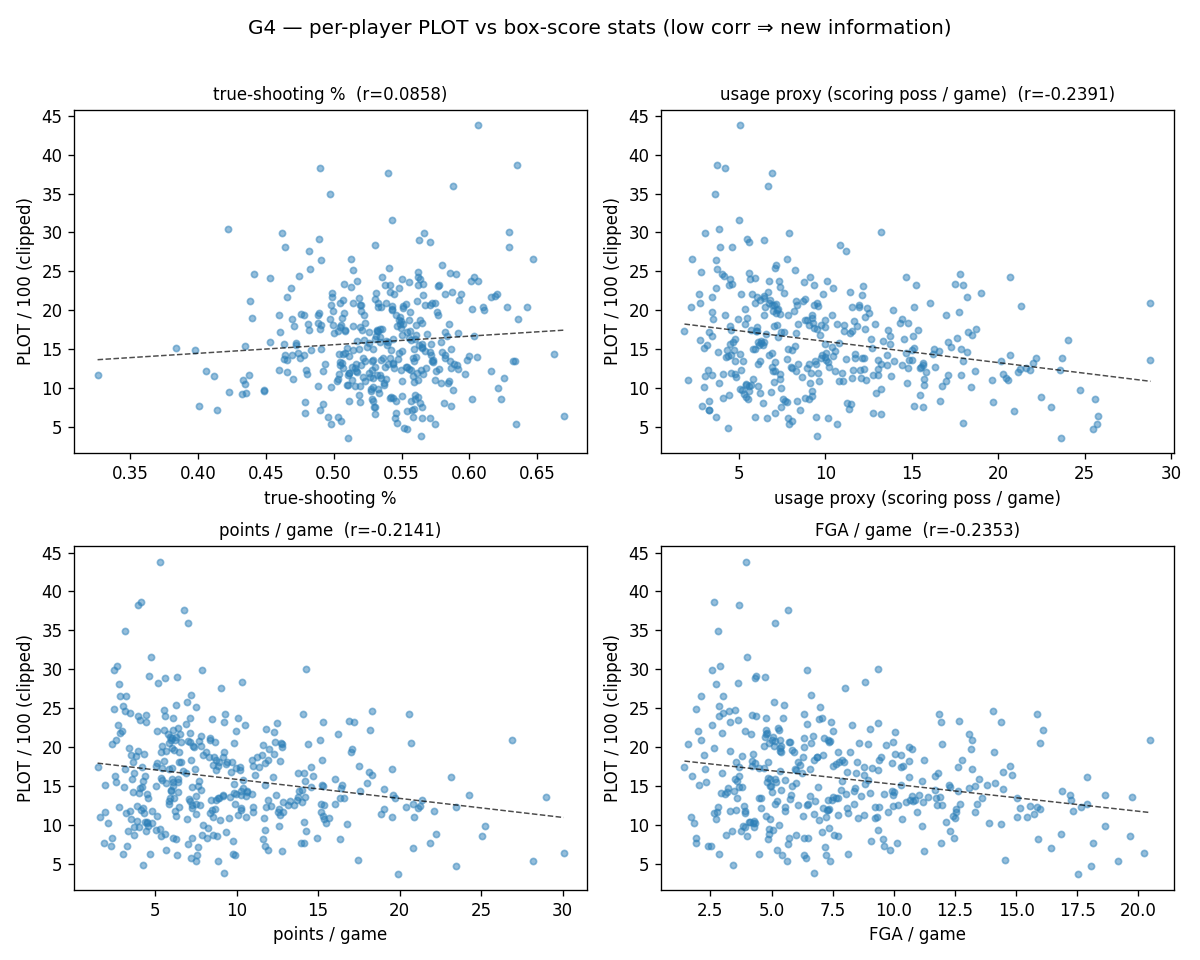
\includegraphics[width=\linewidth]{g4-plot-vs-box.png}
  \caption{G4: \plot{} vs.\ box-score efficiency/usage --- weak to null, i.e.\ incremental information.}
  \label{fig:g4}
\end{minipage}
\end{figure}

\textbf{The leaderboard, and an honest caveat.} Sorted by raw \plot{}, the top is rim-running bigs and
role players (Miles Plumlee, Montrezl Harrell, Kosta Koufos, Willie Cauley-Stein, Hassan Whiteside) and
the bottom is high-usage lead guards (John Wall, Russell Westbrook, Bradley Beal, Kevin Durant). This is
face-valid --- bigs defer open looks; guards take them --- but it is exactly the validity worry: is a big
kicking out an open 18-footer a \emph{bad decision} or correct \emph{deference to role}? G4 establishes
that \plot{} is new information; it does not by itself establish that the information is decision
\emph{quality}. Sections~\ref{sec:g6decomp}--\ref{sec:g6keystone} address this directly. One caution on
the names: split-half reliability is moderate (Spearman--Brown $0.68$ for raw \plot{}, $0.54$ for the
within-role residual; \S\ref{sec:g6decomp}) --- high enough to establish that a real between-player signal
\emph{exists}, but not high enough to pin any single player's value precisely. Individual estimates
carry meaningful sampling noise, so this leaderboard should be read as evidence that the signal is real,
not as an exact ranking of these specific players.

\textbf{Gate G5 (validity conditional on observables).} Three checks (demonstrated on the 42-game
development corpus; these are method properties that transfer): (a) the regret inputs are calibrated
within the open-decision subspace, not just on average (post-pass \epv{} ECE $0.055$, \xpts{} make ECE
$0.040$; near-rim \xpts{} is if anything biased \emph{low}, which would \emph{under}-credit bigs'
passed-up rim looks --- the opposite of the feared bias); (b) selection onto the decision is, as
expected, strong (propensity AUC $0.82$) but driven by \emph{modeled} features (distance and openness ---
\xpts{}'s own inputs), so the metric conditions on the selectors; (c) the per-player ordering is robust to
finishing skill --- a shooter-aware \xpts{} barely reorders the leaderboard (Spearman $0.93$, top-30
overlap $0.80$). The residual threat is selection on \emph{unobservables} (shot difficulty beyond
location and openness), which is irreducible without a counterfactual and is our principal standing
caveat.

% ===========================================================================
\section{What does it measure, and is it real? (Gate G6)}\label{sec:g6}
% ===========================================================================
Everything through G5 is \emph{internal}: regret is the model compared against itself or its own
construction. G6 asks the two questions that decide whether the paper says something true and useful:
\emph{what} does the between-player signal measure (role-of-touch vs.\ within-role decision quality), and
does it predict anything \emph{real} (outcome validity)?

\subsection{Role-of-touch vs.\ within-role decision quality}\label{sec:g6decomp}
Every variant of the metric puts bigs near the top, raising the worry that \plot{} measures \emph{where a
player gets the ball} rather than \emph{how well he decides}. We put a number on it. On the credible set
(153{,}098 decisions, 387 players $\ge 30$), we fit a \textbf{context model} $\text{regret}\sim\text{touch
context}$ (court location, openness, rim distance, three-point indicator, decision kind) with \emph{no}
player identity, out-of-fold by game. The out-of-fold prediction is the \textbf{role} component (the
regret anyone faces in that spot); the residual is the \textbf{within-role} component (how much this
player beats or trails the situation's expectation). We then decompose the between-player variance via the
exact identity $\mathrm{Var}(\text{raw}) = \mathrm{Var}(\text{role}) + \mathrm{Var}(\text{resid}) +
2\,\mathrm{Cov}$.

The result overturns the ``it's just role'' eyeball (Table~\ref{tab:g6decomp}, Figure~\ref{fig:g6decomp}):
within-role decision quality is the \emph{larger} component (within-role share $0.52$ vs.\ role share
$0.29$), and the within-role residual is itself split-half reliable (Spearman--Brown $0.54$,
$p\!\approx\!0$). A leakage check confirms this is genuine: as the role model is strengthened
(weak\,$\to$\,strong), its share rises then plateaus ($0.15\to0.29\to0.32$) while the residual's
reliability stays \emph{stable} ($0.60\to0.54\to0.52$) --- if the residual were merely unabsorbed role, a
stronger role model would eat it; it does not.

\begin{table}[t]
\centering
\caption{\textbf{G6.1 --- role vs.\ within-role decomposition} of between-player variance (208 games,
credible set). The within-role component is the majority of the variance and is reliable; reliability is
stable as the role control strengthens (right), i.e.\ not leakage.}
\label{tab:g6decomp}
\small
\begin{tabular}{lc@{\hskip 2.5em}lccc}
\toprule
Variance share & value & \multicolumn{4}{c}{Leakage sensitivity (role-model capacity)} \\
\cmidrule(l){3-6}
role share              & 0.290 & capacity      & weak & default & strong \\
within-role share       & \textbf{0.525} & role share   & 0.149 & 0.290 & 0.325 \\
cross ($2\,\mathrm{Cov}$) & 0.186 & within-role share & 0.611 & 0.525 & 0.505 \\
$R^2$ role $\to$ leaderboard & 0.505 & residual reliability (SB) & 0.598 & 0.540 & 0.521 \\
\midrule
\multicolumn{2}{l}{raw reliability (Spearman--Brown)} & \multicolumn{4}{l}{0.726} \\
\multicolumn{2}{l}{within-role residual reliability (SB)} & \multicolumn{4}{l}{0.540 \;($p\!\approx\!0$)} \\
\bottomrule
\end{tabular}
\end{table}

\begin{figure}[t]
\centering
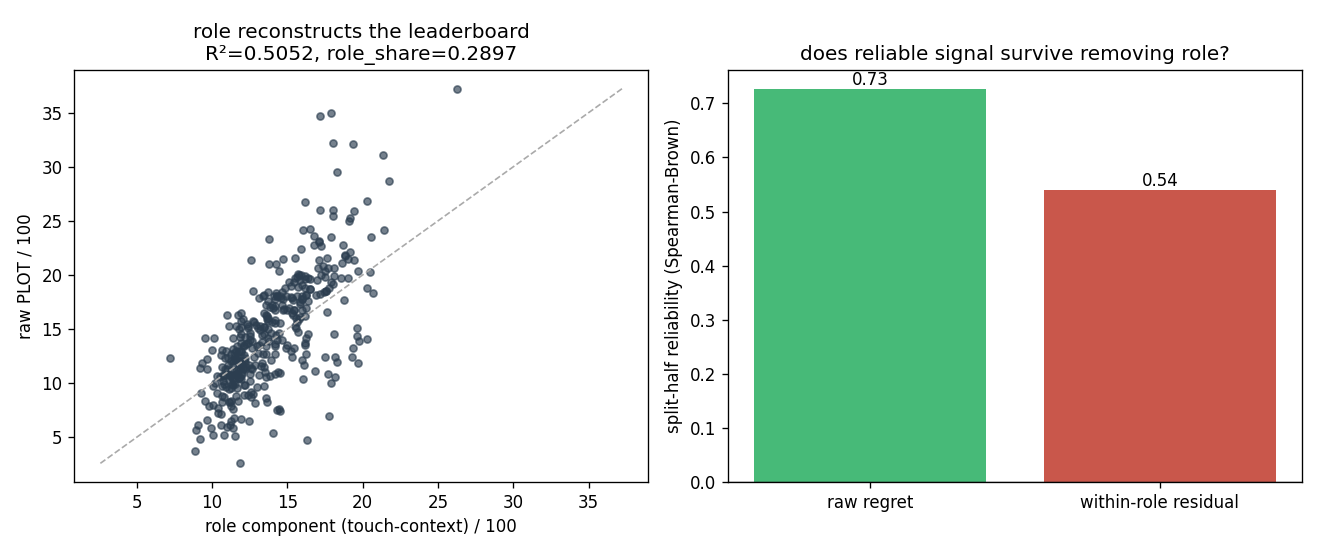
\includegraphics[width=0.92\linewidth]{g6-decomposition.png}
\caption{G6.1. Left: the role (touch-context) component reconstructs about half the raw leaderboard
($R^2=0.51$). Right: a reliable signal \emph{survives} removing role --- the within-role residual is
split-half reliable, so there is real role-adjusted decision quality underneath the role-of-touch.}
\label{fig:g6decomp}
\end{figure}

\subsection{Outcome validity I --- declining your own open look (the keystone)}\label{sec:g6keystone}
This is the one test that is not model-vs-model. The cleanest decision the metric makes is the
\textbf{open look}: a ball-handler with nobody within 4\,ft either \emph{takes} the shot or
\emph{declines} it (passes). We observe realized possession points for \emph{both} choices, so the
counterfactual ``what taking would have yielded'' comes from real shooters at matched situations, not from
the model.

\textbf{Design.} On 208 games we assemble 79{,}877 open-offensive-player decisions: 11{,}365 \emph{takers}
--- the real PBP shots, attributed to the player who actually shot (so the benchmark is the shot's own
realized points) --- and 68{,}512 \emph{decliners} (open ball-handlers who passed). The benchmark $S$ is
the player's own open-shot \xpts{} (same model on both sides); the outcome $R$ is realized possession
points. We regress $R$ on a \texttt{declined} indicator, $S$, their interaction, and observable controls
--- the model's \epv{} at the decision, location, openness, \emph{seconds into the possession}
(a shot-clock-pressure proxy that also corrects for takers acting later than decliners), and period ---
plus team fixed effects, with a \textbf{game-cluster bootstrap} so inference respects within-game
dependence. The validity signature is that the cost of declining is positive and \emph{grows} with $S$.

\textbf{Result (Table~\ref{tab:keystone}, Figure~\ref{fig:keystone}).} It is. Net of observables, clock,
and team, declining an open look costs $0.112$ points $[0.086,0.137]$ on an average look and $0.193$
$[0.141,0.251]$ on a high-value one ($S\!\approx\!1.45$); the $\texttt{declined}\times S$ interaction is
$-0.231$ $[-0.351,-0.116]$ (the cost grows with look value); and the \emph{raw} cost runs from
$\approx\!{-}0.005$ for a bad look (declining it is free --- correct, and cheap) to $\approx\!+0.42$ for a
great one. \textbf{The gate passes at the decision level.}

\textbf{Why it is not an artifact.} (i) \emph{Dose-response}: a pool-composition confound would be flat in
$S$; this is sharply increasing. (ii) \emph{Turnover exposure ruled out}: restricting to possessions that
end in a field-goal attempt (both groups in the same structural position) leaves the high-value cost at
$0.214$ $[0.153,0.278]$ --- declining a good look yields a genuinely \emph{worse shot}, not just turnover
risk. (iii) \emph{Not action-layer mis-typing}: dropping every decliner whose handler took a PBP shot that
possession ($19{,}466$ rows, $\approx\!28\%$) barely moves the estimate ($0.133$ mean / $0.215$
high-value). (iv) \emph{Against selection-on-unobservables}: if decliners passed because they saw a better
play, their realized outcome should be \emph{better}; it is \emph{worse} --- so on average these declines
were not justified by an unobserved superior option (individual ones may be; the bound is on the average,
per the G5 caveat).

\begin{table}[t]
\centering
\caption{\textbf{G6.2 keystone --- realized points lost by declining an open look} (208 games; 79{,}877
decisions). Adjusted for observables, shot-clock proxy, and team fixed effects; $95\%$ game-cluster
bootstrap intervals. Positive $=$ declining costs real points; the negative interaction means the cost
grows with look value.}
\label{tab:keystone}
\small
\begin{tabular}{lccc}
\toprule
Quantity & estimate & 95\% CI & note \\
\midrule
points lost, average look ($S\!\approx\!1.10$)   & 0.112  & $[0.086,\,0.137]$ & $p\!\approx\!0$ \\
points lost, high-value look ($S\!\approx\!1.45$) & \textbf{0.193} & $[0.141,\,0.251]$ & $p\!\approx\!0$ \\
$\texttt{declined}\times S$ interaction          & $-0.231$ & $[-0.351,\,-0.116]$ & cost grows with $S$ \\
\midrule
\emph{robustness:} shot-ending only (no TOs), high-$S$  & 0.214 & $[0.153,\,0.278]$ & survives \\
\emph{robustness:} clean decliner pool (drop $\sim$28\%), high-$S$ & 0.215 & $[0.169,\,0.266]$ & survives \\
\bottomrule
\end{tabular}
\end{table}

\begin{figure}[t]
\centering
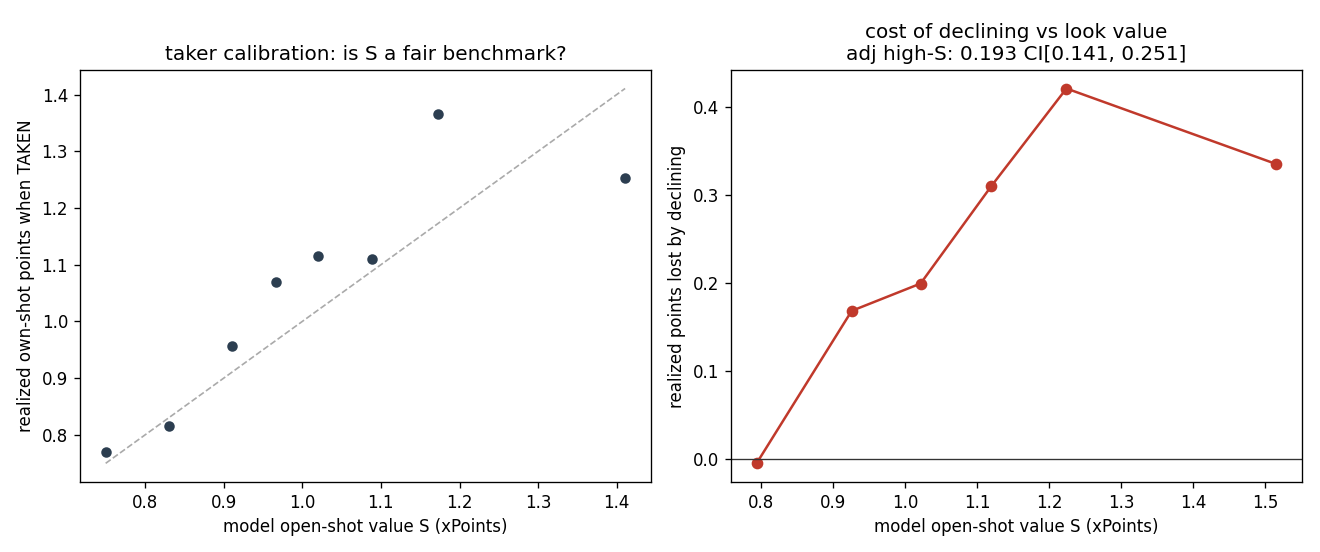
\includegraphics[width=0.92\linewidth]{g6-outcome-validity.png}
\caption{G6.2. Left: taker calibration --- open looks of model value $S$ realize $\approx S$ when actually
taken, so $S$ is a fair benchmark. Right: the realized cost of declining rises with look value --- free
for bad looks, costly for good ones --- exactly the dose-response regret predicts.}
\label{fig:keystone}
\end{figure}

\textbf{Magnitude, honestly.} A 42-game pilot put the high-value cost near $0.47$; the well-powered
208-game estimate is $\approx\!0.19$. The pilot figure was small-sample-inflated. The \emph{sign,
dose-response, and every robustness cut hold}; the effect is real and modest, not large.

\textbf{Magnitude in context.} A fifth of a point per decision invites the question of season-level
stakes, but the aggregate is easy to get badly wrong, and we decline to report a naive one. ``Open''
(no defender within 4\,ft) is a loose, frequently-satisfied condition, so a ball-handler declines an
open look many times per game --- yet most of those declines are \emph{correct} (low-value looks, where
the cost is $\approx\!0$; the signed regret is negative on average, i.e.\ passing usually beats the
contested-spot shot), and the cost concentrates on the minority of \emph{high-value} declines.
Multiplying the per-decision cost by the full decline frequency therefore overstates the stakes by more
than an order of magnitude, and the raw, \emph{unadjusted} bin costs additionally fold back in the
selection the keystone regression removes. A defensible season- or player-level aggregate needs the
per-player frequency of \emph{high-value} open-look declines weighted by the adjusted cost --- precisely
the player-level quantity the cross-fit (\S\ref{sec:g6crossfit}) is built to estimate --- so we report
the validated effect at the decision level and defer the aggregate to that analysis.
% [AUTHOR: once the \S\ref{sec:g6crossfit} cross-fit lands, optionally add a DESCRIPTIVE points/player-season
% aggregate = (per-player count of high-value open-look declines per season) x (adjusted cost ~0.19),
% caveated explicitly as a descriptive aggregate of the metric, NOT validated player-level points.
% Requires the per-player high-S decline frequency from the keystone decision frame (data/processed);
% it is not currently a published gate field, so do not estimate it from the aggregate bin counts.]

\subsection{Outcome validity II --- the open-man myth (a defining negative)}\label{sec:g6asym}
We run the symmetric test for the other half of the credible set: \emph{shooting over a wide-open
teammate}. When a handler has a wide-open ($\ge$6\,ft), frontcourt, reachable teammate, does shooting
over him cost points versus kicking to him? The benchmark $S$ is the kick's value ($0.80\times$ the best
open teammate's \xpts{}); \texttt{declined} now means \emph{shot over the open man}; same controls, team
fixed effects, and bootstrap (56{,}785 decisions: 14{,}761 shot over, 42{,}024 kicked).

It does \emph{not} validate, and the opposite is true (Table~\ref{tab:asym}). The teammate-kick benchmark
is \emph{flat} in $S$ (kick calibration $\approx\!1.0$ regardless of modeled value), the adjusted ``cost''
of shooting over is \emph{negative} ($-0.228$ $[-0.272,-0.190]$: shooting over realizes \emph{more} points),
there is no dose-response (interaction $+0.031$, $p=0.46$), and the gate correctly \textbf{fails}.

\begin{table}[t]
\centering
\caption{\textbf{G6.2b --- shooting over a wide-open teammate does not validate} (208 games; 56{,}785
decisions). The teammate-kick counterfactual is flat in its modeled value, and shooting over the open man
realizes \emph{more} points, not fewer.}
\label{tab:asym}
\small
\begin{tabular}{lccc}
\toprule
Quantity & estimate & 95\% CI & note \\
\midrule
``points lost'' by shooting over, average    & $-0.220$ & $[-0.256,\,-0.185]$ & wrong sign \\
``points lost'' by shooting over, high-$S$    & $-0.228$ & $[-0.272,\,-0.190]$ & wrong sign \\
$\texttt{declined}\times S$ interaction       & $+0.031$ & $[-0.049,\,0.122]$  & no dose-response ($p=0.46$) \\
gate                                          & \multicolumn{3}{c}{\textbf{FAIL} (correctly)} \\
\bottomrule
\end{tabular}
\end{table}

This negative is one of the most valuable results in the project. (i) \emph{It explains why ``score more
decision types'' fails.} An earlier variant that valued every decision against the best open teammate
collapsed into a position sort precisely because this counterfactual is unreliable: an ``open'' man is
often open \emph{because} he is not a threat, so the kick does not deliver its modeled value. We had
diagnosed that by face validity; outcome validity now confirms it. (ii) \emph{It scopes the claim
exactly.} \plot{} is outcome-valid for the decision whose counterfactual is directly observable ---
declining your own open look, whose value is the shooter's own calibrated \xpts{} --- and \emph{not} for
the ``should've passed to the open man'' read, contradicting conventional basketball wisdom. Realness comes
from a clean foundation plus scale plus the one validated decision, not from breadth.

\subsection{Outcome validity III --- player-level cross-fit (de-circularized)}\label{sec:g6crossfit}
The decision-level keystone is non-circular by construction. The \emph{player-level} read --- ``does
\plot{} identify \emph{who} leaves points?'' --- is the prize, and the naive version is circular: correlating
a player's model metric with their own realized shortfall $S-R$ reuses the model's $S$ on both sides
(mechanical) and measures both on the same games. An in-sample version of this correlation is positive
(within-role residual $r=0.33$, $n=373$), but we treat it as exploratory only.

\textbf{Method (the rigorous version).} We remove both leaks with a cross-fit. Split the season's games
odd/even. On one half compute the player's model metric (raw \plot{} and the within-role residual, per
100 decisions). On the \emph{other} half compute their realized points-left as a \textbf{matched-taker
benchmark}: for a declined open look of value bin $b$, the realized cost is
\begin{equation}
  \text{cost} \;=\; \underbrace{\overline{R}^{\,\text{takers}}_{b}}_{\substack{\text{mean realized points of real}\\\text{takers in the same }S\text{-bin}}} \;-\; \underbrace{R}_{\substack{\text{decliner's}\\\text{realized points}}},
\end{equation}
averaged per player. The benchmark is \emph{empirical taker outcomes}, not the model's $S$ (which now only
defines the matching bins), so the two axes share no construction \emph{and} come from disjoint game sets. We run both directions
(metric-on-A/cost-on-B and the swap), pool, and require the pooled within-role correlation to be positive,
significant, and sign-consistent across directions. A positive result is genuine, non-circular
player-level outcome validity; a null is an honest ``decision-level real, player-level attribution not
clean.''

\textbf{Result --- weak, positive, and fragile.} Run over 207 of the 208 games (one game's source
archive was corrupt; immaterial), the cross-fit gives a \emph{modest} signal. Pooled across both
directions ($n=659$ player-halves), the within-role residual correlates with realized points-left at
Pearson $r=0.11$ ($p=0.004$; raw \plot{} $r=0.10$, $p=0.009$), and both directions share the positive
sign, so the pre-registered gate passes. But the result is \emph{fragile}: the two directions disagree
sharply --- model-on-half-B / cost-on-half-A gives $r=0.19$ ($p=0.0005$), while the reverse is
individually \emph{null} ($r=0.05$, $p=0.33$). Read honestly against the in-sample value, the
player-level signal \emph{shrinks} as the circularity and in-sample optimism are stripped out:
$0.33$ (in-sample, shared $S$, same games) $\rightarrow 0.11$ (out-of-sample, empirical taker benchmark).
We therefore report this as \emph{modest, non-circular support} that the metric carries \emph{some}
player-level attribution --- not a clean confirmation. The robust, outcome-validated claim remains at
the \emph{decision} level (\S\ref{sec:g6keystone}); any single player's \plot{} should be read with the
wide uncertainty this and the moderate split-half reliability (\S\ref{sec:skill}) together imply.

% ===========================================================================
\section{The demo}\label{sec:demo}
% ===========================================================================
The value layer and metric are exposed through a chess.com-style possession-review web app (Next.js): an
animated court, an \textbf{eval bar} that rises and falls with \epv{}, and per-decision \textbf{badges}
(Great/Good/Inaccuracy/Mistake/Blunder, thresholded on points left) at open pass-ups. All data are
precomputed to static JSON --- there is \emph{no} model inference in the browser --- so the demo is a thin,
deployable view over the same artifacts the gates use. It makes the abstract metric legible: you watch a
possession and see, frame by frame, where the points went.

% ===========================================================================
\section{Limitations}\label{sec:limits}
% ===========================================================================
We state the ceiling plainly.
\begin{itemize}
  \item \textbf{Scope.} Exactly one decision is outcome-validated --- declining your own open look. Drives,
        and the ``pass to the open man'' read, are explicitly \emph{not} validated (\S\ref{sec:g6asym});
        the metric is a narrow, well-identified instrument, not a general ``decision IQ.''
  \item \textbf{Selection on unobservables.} Conditioning on observables (including the model's \epv{} at
        the decision) bounds selection on \emph{observables}; it cannot rule out that decliners see
        something the tracking does not. The keystone's wrong-direction-for-selection argument bounds this
        on average, but does not eliminate it for individual decisions.
  \item \textbf{Role-of-touch.} About a third of the between-player signal is role-of-touch
        (\S\ref{sec:g6decomp}); the honest object of study is the reliable within-role residual, which we
        isolate but which is harder to communicate than the raw leaderboard.
  \item \textbf{Magnitude.} The validated effect is modest ($\approx\!0.19$ points on a great look). It is a
        real, previously-unmeasured quantity, not a dramatic one. We deliberately do not convert it into a
        season-level aggregate (\S\ref{sec:g6keystone}): the honest one requires a player-level frequency
        the decision-level analysis does not supply.
  \item \textbf{Reliability of individual estimates.} Split-half reliability is moderate (Spearman--Brown
        $0.68$ raw, $0.54$ within-role), which supports the existence of a real between-player signal but
        means any single player's value is estimated with meaningful noise. The leaderboards should be read
        as evidence the signal exists, with uncertainty, not as exact rankings; we do not attach per-player
        intervals because the gate outputs do not currently include them.
  \item \textbf{Corpus representativeness.} The orientation quarantine retains $\approx\!208$ of
        $\approx\!636$ games. This is the right correctness trade-off, but the retained set is not
        guaranteed missing-at-random: if certain arenas, camera installs, or teams produced systematically
        worse tracking and were dropped, the clean corpus may be mildly non-representative of the league.
  \item \textbf{Data.} Public tracking covers half of one season; the 10\,fps action layer can mis-type an
        offensive-rebounded shot as a pass (shown not to drive the keystone, \S\ref{sec:g6keystone}).
\end{itemize}

% ===========================================================================
\section{Conclusion}
% ===========================================================================
Decision quality in basketball is measurable from public tracking, it is a stable and box-invisible player
signal, and --- for the one decision whose counterfactual is directly observable --- it is
\emph{outcome-valid}: players systematically leave real points by declining good open looks, in a
dose-responsive way that survives every robustness cut. The mirror-image read favored by basketball
intuition --- ``pass to the open man'' --- is, by contrast, \emph{not} recoverable from the same data: it
fails the identical test, whether because the open man is open precisely because he is not a threat or
because that counterfactual is too crude to score from tracking alone. That asymmetry is a result in its
own right, and it disciplines the claim to exactly what the data support. The
honest size of the effect is modest, the honest scope is narrow, and the honest object is the
role-adjusted within-role signal --- but it is real, and it is something the box score cannot see. We
release the value layer, the metric, the gate code, and the demo so the result can be checked, extended,
and argued with.

% ===========================================================================
\section*{Reproducibility and data availability}
% ===========================================================================
All models, gates, and figures are reproducible from the released code; the raw tracking data are not
re-hosted but are downloadable from the documented public archives \citep{linou2016movements} via the
included script. Each gate (G1--G6) writes a machine-readable report (calibration tables, bootstrap
intervals, leaderboards) and a figure; the per-player metric and within-role residual are emitted as
columnar tables. The web demo serves precomputed JSON with no in-browser inference.

{\small
\bibliographystyle{plainnat}
\bibliography{refs}
}

\end{document}
